%%%%%%%%%%%%%%%%%%%%%%%%%%%%%%%%%%%%%%%%%
% Short Sectioned Assignment LaTeX Template Version 1.0 (5/5/12)
% This template has been downloaded from: http://www.LaTeXTemplates.com
% Original author:  Frits Wenneker (http://www.howtotex.com)
% License: CC BY-NC-SA 3.0 (http://creativecommons.org/licenses/by-nc-sa/3.0/)
%%%%%%%%%%%%%%%%%%%%%%%%%%%%%%%%%%%%%%%%%

%----------------------------------------------------------------------------------------
%	PACKAGES AND OTHER DOCUMENT CONFIGURATIONS
%----------------------------------------------------------------------------------------

\documentclass[paper=a4, fontsize=11pt]{scrartcl} % A4 paper and 11pt font size

% ---- Entrada y salida de texto -----

\usepackage[T1]{fontenc} % Use 8-bit encoding that has 256 glyphs
\usepackage[utf8]{inputenc}
\usepackage{fourier} % Use the Adobe Utopia font for the document - comment this line to return to the LaTeX default

% ---- Idioma --------

\usepackage[spanish, es-tabla]{babel} % Selecciona el español para palabras introducidas automáticamente, p.ej. "septiembre" en la fecha y especifica que se use la palabra Tabla en vez de Cuadro

% ---- Otros paquetes ----

\usepackage{url} % ,href} %para incluir URLs e hipervínculos dentro del texto (aunque hay que instalar href)
\usepackage{amsmath,amsfonts,amsthm} % Math packages
%\usepackage{graphics,graphicx, floatrow} %para incluir imágenes y notas en las imágenes
\usepackage{graphics,graphicx, float} %para incluir imágenes y colocarlas

% Para hacer tablas comlejas
%\usepackage{multirow}
%\usepackage{threeparttable}

%\usepackage{sectsty} % Allows customizing section commands
%\allsectionsfont{\centering \normalfont\scshape} % Make all sections centered, the default font and small caps

\usepackage{fancyhdr} % Custom headers and footers
\pagestyle{fancyplain} % Makes all pages in the document conform to the custom headers and footers
\fancyhead[L]{Práctica 2}  % Header name
\fancyhead[C]{} % Empty center header
\fancyhead[R]{Fundamentos de la Ingeniería del Software} % Header title
\fancyfoot[L]{} % Empty left footer
\fancyfoot[C]{} % Empty center footer
\fancyfoot[R]{\thepage} % Page numbering for right footer
\renewcommand{\headrulewidth}{0pt} % Remove header underlines
\renewcommand{\footrulewidth}{0pt} % Remove footer underlines
\setlength{\headheight}{10pt} % Customize the height of the header

\numberwithin{equation}{section} % Number equations within sections (i.e. 1.1, 1.2, 2.1, 2.2 instead of 1, 2, 3, 4)
\numberwithin{figure}{section} % Number figures within sections (i.e. 1.1, 1.2, 2.1, 2.2 instead of 1, 2, 3, 4)
\numberwithin{table}{section} % Number tables within sections (i.e. 1.1, 1.2, 2.1, 2.2 instead of 1, 2, 3, 4)

\setlength\parindent{0pt} % Removes all indentation from paragraphs - comment this line for an assignment with lots of text

\newcommand{\horrule}[1]{\rule{\linewidth}{#1}} % Create horizontal rule command with 1 argument of height



%----------------------------------------------------------------------------------------
%	TÍTULO Y DATOS DEL ALUMNO
%----------------------------------------------------------------------------------------

\title{	
\normalfont \normalsize 
\textsc{\textbf{Fundamentos de Ingeniería del Software (2016-2017)} \\ Grado en Ingeniería Informática \\ Universidad de Granada} \\ [25pt] % Your university, school and/or department name(s)
\horrule{2pt} \\[0.4cm] % Thin top horizontal rule
\huge Práctica 3 \\ % The assignment title
\horrule{2pt} \\[0.5cm] % Thick bottom horizontal rule
}

\author{Miguel Ángel Torres López \and Francisco José Ruiz Jiménez \and Francisco Gallego Salido \and Francisco Lopez Rodríguez} % Nombre y apellidos


\date{\normalsize\today} % Incluye la fecha actual

%----------------------------------------------------------------------------------------
% DOCUMENTO
%----------------------------------------------------------------------------------------

\begin{document}

	\maketitle % Muestra el Título
	
	\newpage %inserta un salto de página
	
	\tableofcontents % para generar el índice de contenidos
	
	\listoffigures
	
	\newpage
	
	\section{Diagramas de conceptos}
	
	\subsection{Administración de usuarios, gestión de perfil y gestión de comunicaciones e incidencias}
	
	\begin{itemize}
		\item \textbf{Problema:} los administradores necesitan poder gestionar la actividad de los usuarios del sistema. Los usuarios podrán solicitar registrarse y aquellos que ya dispongan de un registro podrá realizar acciones de gestión sobre su cuenta como gestionar su perfil además de acciones usuales relacionadas con la mensajería.
		\item \textbf{Conceptos:} usuario, usuario registrado, administrador, sistema, mensajes, denuncia.
		\item \textbf{Relaciones: } 
			\begin{itemize}
				\item Los usuarios no registrados podrán solicitar un registro.
				\item Los usuarios registrados podrán gestionar su perfil.
				\item Los usuarios registrados podrán establecer la forma de pago a través del sistema.
				\item Los usuarios registrados podrán añadir o eliminar vehículos en su cuenta.
				\item Los usuarios registrados podrán realizar acciones usuales de mensajería.
				\item Los usuarios registrados podrán poner denuncias explicando el motivo de ella.
				\item Los administradores podrán gestionar las cuentas de los usuarios registrados.
			\end{itemize}
	\end{itemize}
	
	\begin{figure}[H]
		\centering
		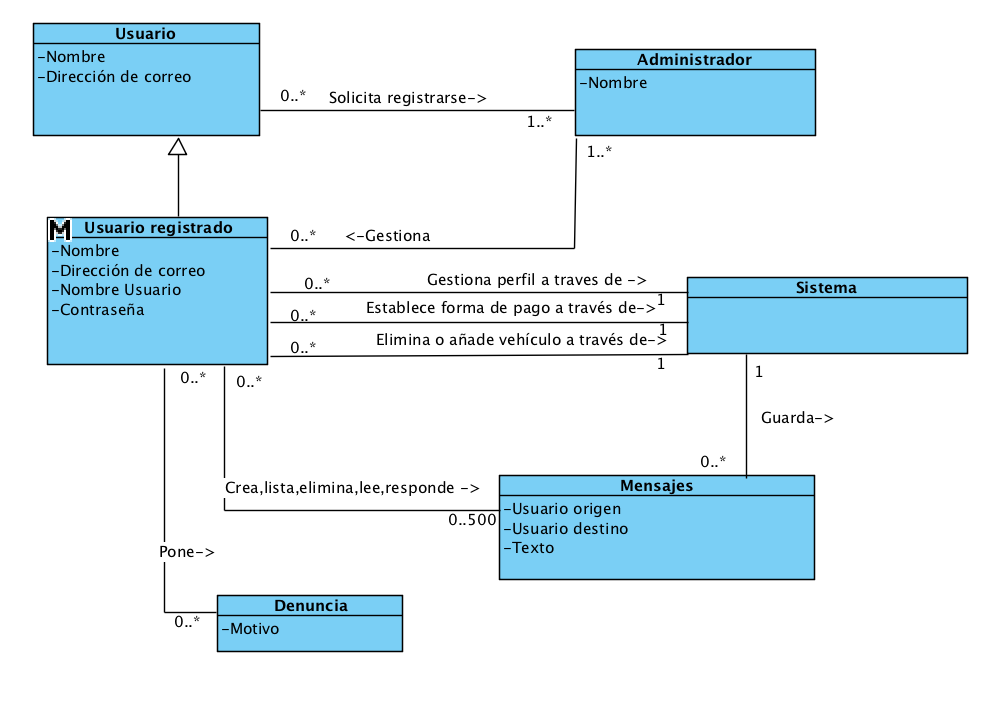
\includegraphics[width=1\linewidth]{img/MC-primero_segundo_quinto_diagrama}
		\label{fig:mc-primerosegundoquintodiagrama}
	\end{figure}

	\subsection{Gestión de viajes y alquileres}
	
	\begin{itemize}
		\item \textbf{Problema: } los usuarios deben de poder realizar gestiones sobre sus planes de viaje y vehículos en alquiler además de poder solicitar y hacer uso de ofertas de otros usuarios. Deberá haber un temporizador que oculte alquileres ya caducados.
		
		\item \textbf{Conceptos: } vehículo, solicitud, plan de viaje, usuario, temporizador, usuario curiosete, alquiler, viaje, openStreetMap, oferta.
		
		\item \textbf{Relaciones: }
			
			\begin{itemize}
				\item Los usuarios podrán ofertar y cancelar alquileres de vehículos y viajes.
				\item Los usuarios podrán solicitar y cancelar solicitudes de viaje.
				\item Los usuarios podrán aceptar o rechazar solicitudes de viaje.
				\item El temporizador deberá ocultar alquileres de vehículos ya caducados.
			\end{itemize}
		\end{itemize}
	
	\begin{figure}[H]
		\centering
		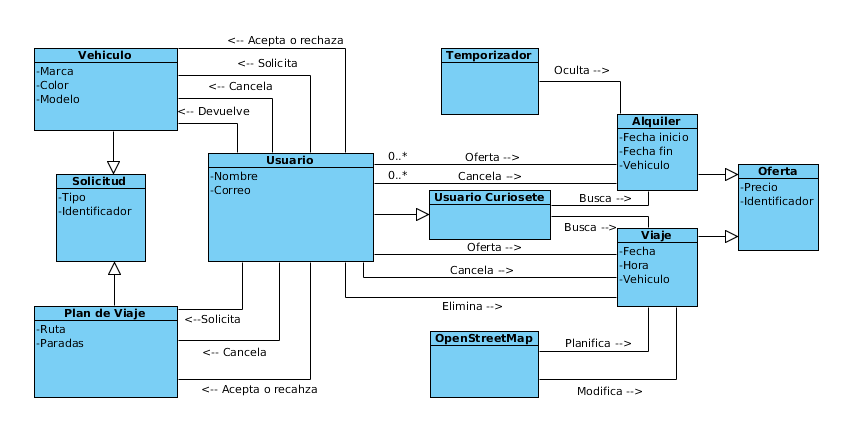
\includegraphics[width=1\linewidth]{img/Gestion_alquileres_viajes}
		\label{fig:gestionalquileresviajes}
	\end{figure}

	
	
	\section{Diagramas de secuencia}
	
		\subsection{Administración de usuarios}
		
		\begin{enumerate}
			\item Un usuario registrado tiene que identificarse en la plataforma.
			\item El administrador puede dar de baja a un usuario.
			\item El administrador puede consultar la información de un usuario.
			\item Un usuario puede registrarse en la plataforma.
			\item Un usuario puede dar de baja su registro en la plataforma.
		\end{enumerate}
		
		\begin{figure}[H]
			\centering
			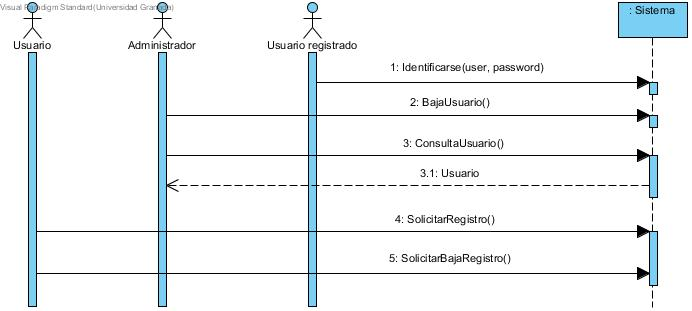
\includegraphics[width=1\linewidth]{img/secuencia1}
			\label{fig:secuencia1}
		\end{figure}

		\subsection{Gestión de perfil}
		
		\begin{enumerate}
			\item Un usuario puede modificar la visibilidad de su perfil.
			\item Un usuario puede introducir datos en su perfil.
			\item Un usuario puede modificar su perfil.
			\item Un usuario puede consultar el perfil de otros usuarios.
			\item Un usuario puede establece la forma de pago que va a utilizar.
			\item Un usuario puede establecer la forma de cobro que desee.
			\item Un usuario puede añadir vehículos a su perfil.
			\item Un usuario puede eliminar vehículos a su perfil.
		\end{enumerate}	
		
		\begin{figure}[H]
			\centering
			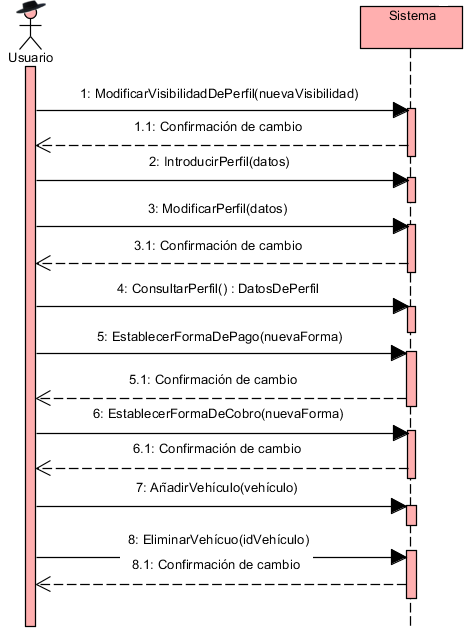
\includegraphics[width=0.8\linewidth]{img/GestionDePerfil}
			\label{fig:gestiondeperfil}
		\end{figure}

		
		\subsection{Gestión de viajes}
		
		\begin{enumerate}
			\item Un usuario curiosete puede buscar un plan de viaje indicando sus preferencias.
			\item Un usuario puede consultar la valoración de un conductor.
			\item Un usuario puede planificar un viaje.
			\item Un usuario puede modificar un viaje planificado previamente.
			\item Un usuario puede eliminar un plan de viaje que había sido planificado previamente.
			\item Un usuario puede ofrecer un viaje ya planificado para que este sea visible a los demás usuarios y estos puedan solicitarlo.
			\item Un usuario puede cancelar una oferta de plan de viaje.
			\item Un usuario puede solicitar un plan de viaje disponible.
			\item Un usuario debe de seleccionar una forma de pago tras solicitar un plan de viaje.
			\item Un usuario puede aceptar o rechazar una solicitud recibida de un plan de viaje.
			\item Un usuario puede consultar la valoración de un acompañante del viaje.
			\item Un usuario puede cancelar una petición realizada de un plan de viaje.
			\item Un usuario debe de finalizar un viaje tras el fin de este.
			\item Un usuario debe realizar el pago de un viaje tras su finalización.
			\item Un usuario puede valorar a los acompañantes de un viaje.
			\item Un usuario puede valorar un viaje realizado.
		\end{enumerate}

		\begin{figure}[H]
			\centering
			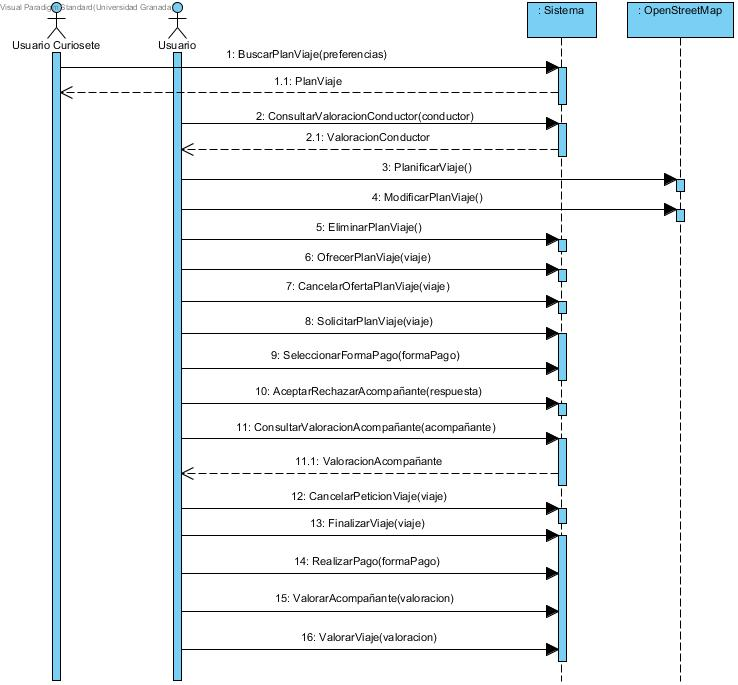
\includegraphics[width=1\linewidth]{img/secuencia2}
			\label{fig:secuencia2}
		\end{figure}
		
		\newpage
		\subsection{Gestión de alquileres}
		
		\begin{enumerate}
			\item Un usuario curiosete puede buscar una oferta de alquiler indicando sus preferencias.
			\item Un usuario puede consultar la valoración de un alquiler.
			\item Un usuario puede ofertar el alquiler de un vehículo.
			\item Un usuario puede cancelar la oferta de un alquiler de vehículo.
			\item Un usuario puede solicitar un vehículo que este en alquiler.
			\item Un usuario debe seleccionar la forma de pago tras solicitar un vehículo.
			\item Un usuario puede cancelar una solicitud de vehículo.
			\item Un usuario puede aceptar o rechazar una petición de vehículo.
			\item Un usuario puede consultar la valoración de un aspirante.
			\item Un usuario debe devolver el vehículo tras finalizar el periodo de alquiler.
			\item Un usuario debe realizar el pago del alquiler tras la devolución del vehículo.
			\item Un usuario puede valorar el uso.
			\item Un usuario puede valorar el alquiler.
			\item El temporizador oculta las ofertas caducadas.
		\end{enumerate}
		
		\begin{figure}[H]
			\centering
			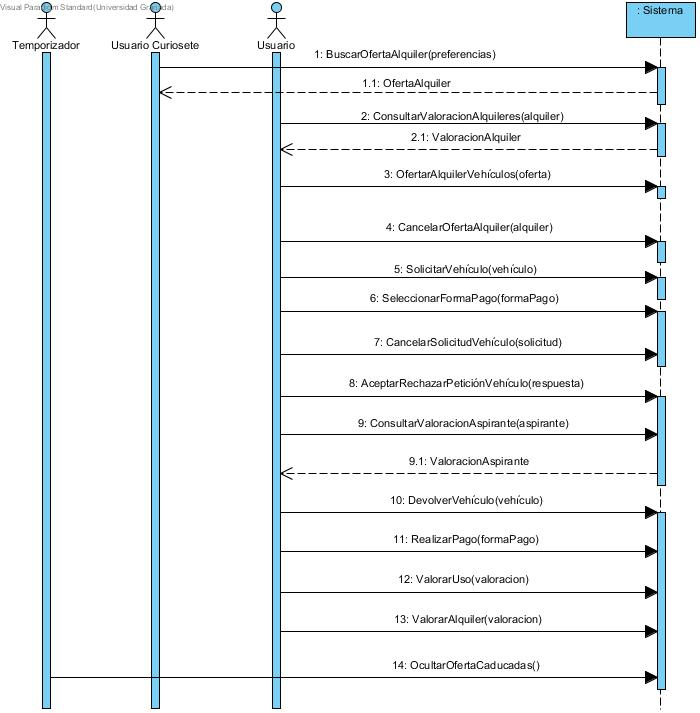
\includegraphics[width=1\linewidth]{img/secuencia3}
			\label{fig:secuencia3}
		\end{figure}
		
		\subsection{Gestión de comunicaciones e incidencias}
		
		\begin{enumerate}
			\item Un usuario puede crear y enviar mensajes a otros usuarios.
			\item Un usuario puede consultar la lista de mensajes.
			\item Un usuario puede leer sus mensajes.
			\item Un usuario puede borrar mensajes.
			\item Un usuario puede responder mensajes.
			\item Un usuario puede declarar la incomparecencia de otro usuario.
			\item Un usuario puede denunciar la no disponibilidad de recursos.
			\item Un usuario puede denunciar el mal uso de un recurso.
			\item Un usuario puede denunciar el impago de otro usuario.
		\end{enumerate}

		\begin{figure}[H]
			\centering
			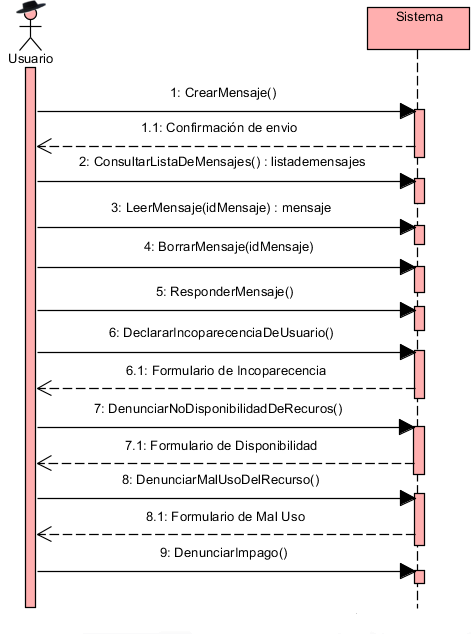
\includegraphics[width=0.8\linewidth]{img/GestionDeComunicaciones}
			\label{fig:gestiondecomunicaciones}
		\end{figure}


\end{document}


